

%_________________________________________________________________________________
\chapter{Outlook}

This section explores further developments of the model. The first section focuses on how the phenotypic plasticity is modelled, and how alternative approaches can help understand this process and its effects. The second part of this discussion describes ways to widen the scope of the model by taking advantage of the already existing resources.

\section{How to model phenotypic plasticity? }

The framework developed during this project constitutes a step forward in the modelling of the phenotypic plasticity. It integrates the idea of streategic plasticity \parencite{bradshaw_evolutionary_1965, dewitt_expanding_2016} within a phenotypic space drawn by allocation trade-offs that allows the modelling of diverse community. But the limitations shown by the current implementation reveals that the question of the modelling of the phenotypic plasticity is not resolved. While the question of the plastic dimension will always be present when modelling phenotypic plasticity, the main interrogations revolves around the drivers and the use of the information. 

%how do we think about plasiticity: this model is a step forward, despite seen as a ...

\paragraph{Explore the limits}

The question of the plasticity as a strategy trait was not fully explored despite being a centre point in the design of the model. This plasticity as a strategy, rather than a growing function, expresses the idea the existence of limits that justify that not all species are plastic \parencite{dewitt_costs_1998 ,  van_kleunen_constraints_2005, valladares_ecological_2007, auld_re-evaluationg_2009}. These plastic, in addition to be observed in natural systems, are also needed in the context of the model to avoid convergence and Darwinian demons. These limits are numerous and can be separated in multiple categories: actual limits that prevent an effective plasticity that increases reliably the fitness, and costs that negate the fitness gain provide by the changes in phenotype.\cite{valladares_ecological_2007} also distinguish internal limits and ecological limits, but these are not always clearly circumscribed and quantified. The internal costs must be implemented in the model, to avoid unnatural behaviours and explore emergent properties. The ecological limits, on the other hand should emerge from the mechanisms implemented. For example, the variability of the climatic conditions, should favour the selection or species with high plasticity in the current implementation of the model, if it is not too variable and impredictable. This could be tested with simulations with two axes of treatment: temporal variability and auto-correlation. Mechanistic approaches, informed by the knowledge of the plant biology, allow the consideration of internal limits such as morphological limits \parencite{valladares_ecological_2007}, as implemented in \cite{maire_plasticity_2013} or \cite{lohier_analyse_2016}, and to a lower extend by the allocation trade-off in \model . But as observed in this implementation, the allocation trade-off does not take into account the whole extent of the morphological limits, and further work is needed to quantify those. The mechanistic model also prevent unrealistic plasticity by the natural limitation of the phenotype's flexibility \parencite{forsman_rethinking_2014}. The balance between the growth and the turn-over must be finely calibrated to capture this limitation of the plasticity that can cause lags in the plastic responses \parencite{dewitt_costs_1998}. % calibration ! ! !
 Other cost costs are harder to quantify, such as the maintenance, acquisition and production costs. Methodologies are proposed to study the potential cost of plasticity \parencite{dewitt_costs_1998, valladares_quantitative_2006}, they have found limited effects in natural systems \parencite{van_kleunen_constraints_2005}, despite potential effects in a context of low genetic variation \parencite{dechaine_constraints_2007}. The difficulty to quantify globally the plasticity cost comes from the difficulty to disentangle the different forms of cost \parencite{murren_constraints_2015}, the potential cost of homoeostasis \parencite{van_kleunen_progress_2007}  and statistical limitations \parencite{auld_measuring_2011}. These difficulties are illustrated by the implementation of the cost of the plasticity in \model . The production cost, relative to the expression of an alternative phenotype different from the current phenotype, can intuitively be expressed as a function of the phenotypic distance between the two phenotypes \cite{valladares_quantitative_2006}. But the choices relative to the computation of this distance are numerous and hard to justify: should the current or the 'default' phenotype be the point of references, what axes are considered (composite traits such as the  SLA, individual traits, morphological or chemical traits) and their relative importance, etc...
The quantification of the costs of plasticity represents a challenge that requires progress and collaboration from the empirical studies, modelling approaches and statistical method. This challenge is crucial for the quantitative estimation of the importance of the plasticity on the community dynamics.
  % The value of a model like \model resides in its capacity to run simulations to test the validity of these hypotheses. 
%
%The limit of the predictability, variability and uncertainty
%
%The reliability of the external cues about the future stress is a limit often identified.  This uncertainty can ban on factor that explains the failure of the \textit{plastic-optimisation} algorithm to consistently increase plant fitness. The error in the projection of realised conditions (because of unreliable cues, wrong driving rule, or competition interactions)   % non symetry in the fitness landscape, benefit risk, optimum and stability.
%
%Between optimisation and stability
%
%competition % requires better knowledge of how interactions work there , with approaches similar to tilman, and see how plasticity can affect them (
%
%and other traits 

\paragraph{A molecular-inspired plasticity}

As mentioned, having a modelling approach closer to the molecular mechanisms would explicit some internal limits of the plasticity. In particular, the use of reaction norms would capture the complexity of the mechanism and the difficulty to integrate multiple signals. The prediction capacity would also be limited by the form of these reaction norms. It also implies a high number of species specific parameters, increasing with the number of stresses considered. These arguments were invoked to justify the integrative approach of the model, but make the mechanism more grounded in the reality.

The advantages provided by a molecular-inspired approach go beyond the explicit limitations. Species specific reaction norms would at the same allow more amplitude in the plasticity responses, but also more diversity \parencite{kichenin_contrasting_2013, wellstein_intraspecific_2013}. This method could easily model contrasted responses between avoidance and tolerance as a function of the global plant strategy, \parencite{perez-ramos_tradeoffs_2013} or the available information \parencite{heger_light_2016}. This diversity in response also allows responses outside the trade-offs. Despite evidences of an economic spectrum at the intra-specific scale \parencite{hu_novel_2015, fajardo_intraspecific_2018}, the leaf economic spectrum does not totally control intra-specific variations \parencite{fajardo_intraspecific_2018} and plastic responses do not have the same objectives \parencite{ryser_consequences_2000}. Molecular approaches should still be constrained by morphological and physiological limits, but not necessarily the same that determine the default plant strategies.

% about memory
A molecular-inspired plasticity, could better mimic the accumulation of stress molecules, that increase the amplitude of the plastic response following a second stress signal \cite{crisp_reconsidering_2016}. This type of mechanisms also greatly illustrates the idea of species memroy against the plant experience \sidenote{or \textit{memory} as named in \cite{crisp_reconsidering_2016}, but \textit{experience}is prefered here to avoid ambiguity.}. The idea of stress levels, competing with the growth \cite{herms_dilemma_1992} and eventually other forms of stress (frost, grazing, drought , etc...), was originally planed for the model, but the number of stresses were limited to avoid a too complex model. This limitation to resource-related stresses also allowed the simplication of the plastic driving mechanism with the use of an integrative function. But this idea of competing stresses, based on melcular-inspired plasticity and plant-specific experience is attractive and should unlock a better understanding of the plasticity mechanisms.

%more molecular approach, to have stronger patterns, and avoid observed limitations

%break the trade-offs, not the same mechanisms (information, time sale, objectives)
%avoidance and resistance : variability in response.

\paragraph{Plasticity, epigenetics \& genetics}

The framework developed during this work establishes the plasticity as a strategy, but also includes the perception of external conditions as components of the overall strategy. These driving external conditions change at the scale of the season, justifying phenotypic plasticity, but also follow larger trends between seasons. These trends can lead to a gap between the default phenotype, or species memory of the external conditions \sidenote{as tthe two are linked in the model. Here I use these two terms to identify the species stratgy expressed by the default phenotype, but depending on the species memory for the external conditions.}, and the average optimum phenotype, or average experience conditions. This gap can be captured by plants, even in the context of an adaptive phenotype, by the comparison of either the experienced conditions, the stress levels and direction or the plastic responses, to respectively the species memory, the absence of stress or the average phenotype. The quantitative perception of this gap, expressed by directed plastic responses, can be transmitted to following generation to better fit to the general trend in the external drivers. This form of heritability ban have a great effect on the community dynamics, particularly on their ability to cope with climate change. The heritability in intra-specific variable traits provides resilience to environmental disturbances and stabilise trait patterns \cite{barabas_effect_2016}.

The heritability of driven changes in phenotypes also makes sense in a molecular perspective. Indeed, a lot of plasticity mechanisms involve epigenetic inheritable mechanisms, such as histone modifications, DNA methylation or sequence modification \cite{nicotra_plant_2010}.

% genetics and plasticity as a genetic traits that can be altered.
The heritability of driven changes in phenotypes, or driving traits such as the species memory, differ from random mutation and selection. However, the evolutionary process of mutation and selection of traits could lead to a greater understanding of the plasticity processes. First, it would allow the comparison between the dynamics of genetic and epigenetic modifications, and their relative impact on the community dynamics. If genetic modifications can lead to a diversification of the community, epigenetic modifications certainly increases the resilience to rapid environmental shift. Second, the incorporation of genetic algorithm would allow the selection of effective forms of plasticity, especially if the plastic responses are determined by reaction norms with species-specific parameters. The selection of the reaction norm forms, and the study of the species specific parameter distribution can greatly improve our understanding of this mechanisms.

The coexistence of epigenetic and genetic control can lead to particular phenotypic distribution. It may be important to consider such distributions to understand plasticity strategies at the scale of the species \parencite{dewitt_expanding_2016}.


\begin{figure*}%[tb]
    \classiccaptionstyle
\sidebysidecaption{0.5\textwidth}{0.4\textwidth}{%
    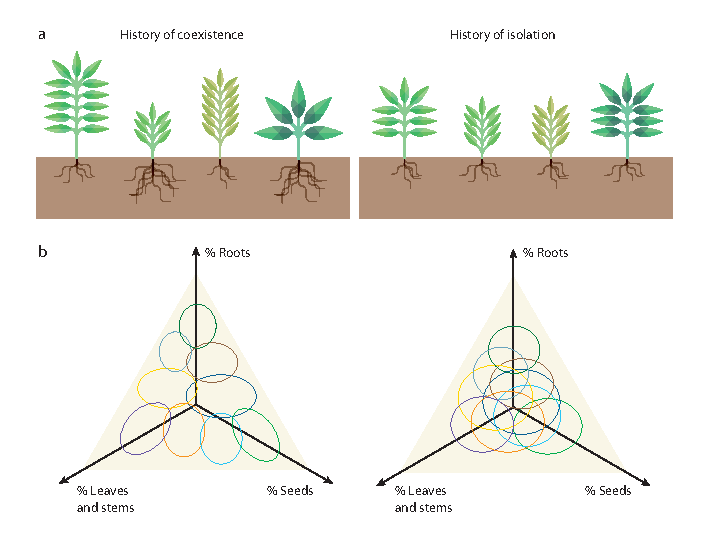
\includegraphics[width=1\linewidth]{./3_Synthesis/graphics/niche_shift.pdf}%
}{
  \caption[ Evolutionary niche shifts.]{ Evolutionary niche shifts. a) \cite{zuppinger-dingley_selection_2014} find that, when plant species are grown in a common environment, those that have a history of selection in diverse communities develop greater differences in traits than species that have a history of isolation. b) This idea feeds into our understanding of how evolutionary history influences the ecological interactions of species that compete for growth factors such as soil nutrients, light and space. All species face trade-offs. For instance, biomass that is allocated to obtaining soil nutrients (roots) cannot be used to obtain light (leaves and stems) or to disperse to open sites (seeds). Graphically depicted, the resulting ‘trade-off surface’ (triangles) represents all possible ways in which plant species (ellipses) can allocate their biomass. A history of selection in diverse communities results in greater interspecific differences (less overlap of
ellipses) and more specialization (smaller ellipses) than a history of isolation. From \cite{tilman_diversity_2014}, reproduced with the permission of Springer, license number: 	
4386020602501.}
  \label{fig:niche_shift}
 }
\end{figure*}

The epigenetic changes, that link the experience of the external conditions with species strategies and transmits this information to following generations may play an important role in the character displacement observed in empirical experiments \parencite{zuppinger-dingley_selection_2014}. The ability of coexisting species to express contrasted phenotypes increasing the biodiversity may rely on the phenotypic plasticity\parencite{roscher_contrasting_2015}, but epignetic processes may play a role in the stability of this mechanisms and a long-time effect on biodiversity \parencite{tilman_density_2014}.



% heritaibility and effects

% link with molecular level mechanisms nicotra and 
%
%The previously mentioned concept of an individual experience competing with a 
%Plasticity as a strategy: genetic dyn + extend the discussion of the limits
%
%heritability: how can it be transfert, wht should be transferred, effect of this heritability (dewiit and barabas)

\paragraph{It is about information}

The development of the implementation of the phenotypic plasticity listed above introduce a lot of complexity and computational costs. Another approach, at the conceptual end of the modelling approaches, is to consider the external resources and stresses as information to solve an investment problem. Once the gains and cost function established, the reliability of the information, the uncertainty and the risks can be computed similarly as in other systems such as economic optimisation problems. This would extend the view of the plant physiology as an economic problem \parencite{westoby_time_2000, wright_worldwide_2004, mcmurtrie_leaf-trait_2011}. Such approach relies on two sides: an explicit and precise description of cost and gain functions, and a prediction of the controlling variables. The former is relies on a good understanding of plant physiology, and current knowledges allow a good representation of these processes, but the costs of the plasticity need to be better quantified as already highlighted. The reliability of the information for the prediction of the future conditions has already been pointed out in multiple studies \parencite{ dewitt_costs_1998, auld_re-evaluating_2009, richter_phenotypic_2012}. The inability of a plant to consider the cost of being wrong is one argument explaining the low performances observed in \textit{plastic-optimisation} simulations, despite a more flexible plastic allocation allowing for a better exploration of the phenotypic space. The productive, but less efficient phenotypes selected by this algorithm do not authorise errors in the prediction of the resource availability because of their higher sensitive to unbalanced organ activities. This particular case could be solved by the evaluation of alternative projection at the same time multiple phenotypes are evaluated. While it would increase the computational cost by increasing the dimension of the space explore, better implementation and exploration algorithm could compensate for this downside. In addition, the overall complexity of the model would almost stay the same as it would require only one additional model to weighted the chance to optimise the fitness with the risk of unstable phenotypes in case of uncertain prediction.

More advanced learning processes can be investigated to model the phenotypic plasticity. The concept of adaptive learning is also a path to explore for the development of the phenotypic plasticity. As genetic algorithm evaluate the success of a strategy by a fitness function at the end of a cycle, individuals could evaluate the performance of plastic response strategies after a few days. The driver of the plasticity resides in the evaluation of the current phenotype for the current and future conditions, in order to eventually develop alternative phenotypes if the performance in not satisfactory\sidenote{this sound finalist, but I use this formulation to emphasise the step of the evaluation of the phenotype. This evaluation can take the form of a concentration in a certain stress molecule in a less perspective approach.}. Therefore, in the context of plastic phenotype, the evaluation step quantifies at the same time the success\sidenote{any relevant fitness proxy.} of the current phenotype, but also the success of the plasticity that lead to this phenotype. The plastic strategy is evaluate through the improvement in the phenotype's success, rather than the absolute value of the fitness function. This relative change in fitness must also consider the external stress intensity to avoid penalising well performing plastic strategies under more intense stress. This evaluation of the plasticity strategy allows to adapt the parameters of the plastic response itself, but also the variables required to build the need projection of condition, increasing the confidence and reducing the risks of the uncertainty mentioned above. This approach however makes sense under a complex and performing prediction algorithm, and may not fit the scope of the current model that focuses on community dynamics. Specific deigns of plastic plant models will be required to explore this track.

%alternative approach: prediction and the information available

%adaptive learning

%stress also informs on how 


\section{Beyond the simple community}

The previous part of the perspectives that emerge form this work focuses on improvements of the implementation of the phenotypic plasticity. But the model already offers a new tool to explore the effects of the phenotypic plasticity on grassland communities that have only been scratched.

\paragraph{The role of the climate}

take advantage of the already present information,
build a better calibration -> more precise, prediction

consider the already implemented feature: frost stress and grazing/cutting.

\paragraph{About ecosystem services}

with better calibration, better quantification of measure traits (that were a bit put on the side here) and more specific results (site and weather)

Link the properties together

\paragraph{The meta-community dynamics}

Can have a pretty good role: reinforce or mitigate patterns 
already possible

landscape dynamics

invasion and critical transitions

\paragraph{The climate change}

precise, calibrated model, closer to real systems to link to ES, with proper landscape dyns.

management scenarios and climate scenarios, intreracton \cite{deleglise_drought-induced_2015}

fantasised view of the model but this exitment makes us work.

%Further reading, thinking and rambling about what's developped in the papers.
%
%%\section{Plasticity and resistance to climatic events}
%
%%\section{•}
%
%\subsection{Better calibration}
%
%Better implementation rcpp or data table struture, plasticity mech, to allow bayesian and pattern-oriented calibration. A lot of species and a lot of parameters. Difficult exercice. But strategies should be limited by functions and trade-off, just need to calibrate shared (process related) parameters and not species specific (strategic) paramters. This is what allows the modelling of diverse community. 
%
%
%\section{Competition and feedback}
%This document focuses on how the plant are doing with the given resources (arrow in fig in margin). However, a key element in competition and resource dynamics (point that separate Tilman appraoches from Chesson) is the impact of plant on resource (fig in margin). Both are fundamental for the understanding on plant interactions, and I argue that understanding the former is necessary to understand the later and have a global view on plant competitive interactions on resources. blablabla competition experiments, resistance to resource shortening (Tilman) and relative homogeneity of resource (homogeneous in influx, content, starting pool, ... ?). Using the term homogeneous allows to use fixed terms and processes, while to me there is a ambiguity around competition that can be seen as: (1) the impact on growth, (2) the winner out of a competitive scenario (with resource shortening). In this later case, the approach of part 4 (?) has limited interpretation since they are not competing. We can intuiitively imagine (from our understanding of model's functioning) that  there is a hierarchical effect on growth, but that is probably reversed in case of (1) shared resource pool (big plant may have access to bigger resource pool in open environment), (2) sufficiently quick resource shortening to lead to death events.\\
%
%in margin: figure resource and interaction.\\
%figure competition decomposition of fitness (growth and survival), and growth related to resource pool (try to have graph approach).
%
%competition change vegetation response to climate change \parencite{van_loon_how_2014}
%
%transitivity and competition \cite{levine_beyond_2017} Could it emerge from the current implementation of \model ? Is it stable with plasticity ?
%
%
%\section{Extend to climate change effects}
%
%How plasticity actually affect the effects of climate change: mitigate or amplify, risk of critical transition.
%
%drought resistance experiments to be done.
%
%Higher diversity: higher risk of invasion?
%
%Take advantage of simulated scenarios of climate change.
%
%\section{Going forward: epigenetic and heritability}
%
%fundamental knwowledge 
%
%effect of heritability and genetic effects (evolutionary perspective) Bring the two perspective together. \cite{scheiner_genetics_1989}
%
%Bayesian model of dev. \cite{stamps_bayesian_2016} Talked about the difficulty to match reaction norms with systemic plasticity: evolutionay bayesian approach to species specific reaction norms.
%
%Epigenetic variation creates potential for evolution of plant phenotypic plasticity \cite{zhang_epigenetic_2013}
%See also \cite{dewitt_expanding_2016} for higher moment of reaction norms controlled by genes